\chapter{Using and Modifying the Data Structure}
\label{chapter:data_structure}
MAUS operates on data in discrete blocks, known as spills, with one spill representing the particle burst generated by one dip of the MICE target. The major part of the MAUS data structure therefore is a tree of which each entry corresponds to the data associated with one spill. The spill is separated into three main sections: the MCEventArray contains an array of data each member of which represents the Monte Carlo of a single primary particle crossing the system; the ReconEventArray contains an array of data each member of which corresponds to a particle event (i.e. set of DAQ triggers); and the DAQData corresponds to the raw data readout. Additionally there are branches for reconstructed scalars, which are handled spill by spill and EMR data, which also read out on the spill rather than event by event.

\begin{figure}[!htb]
\centering
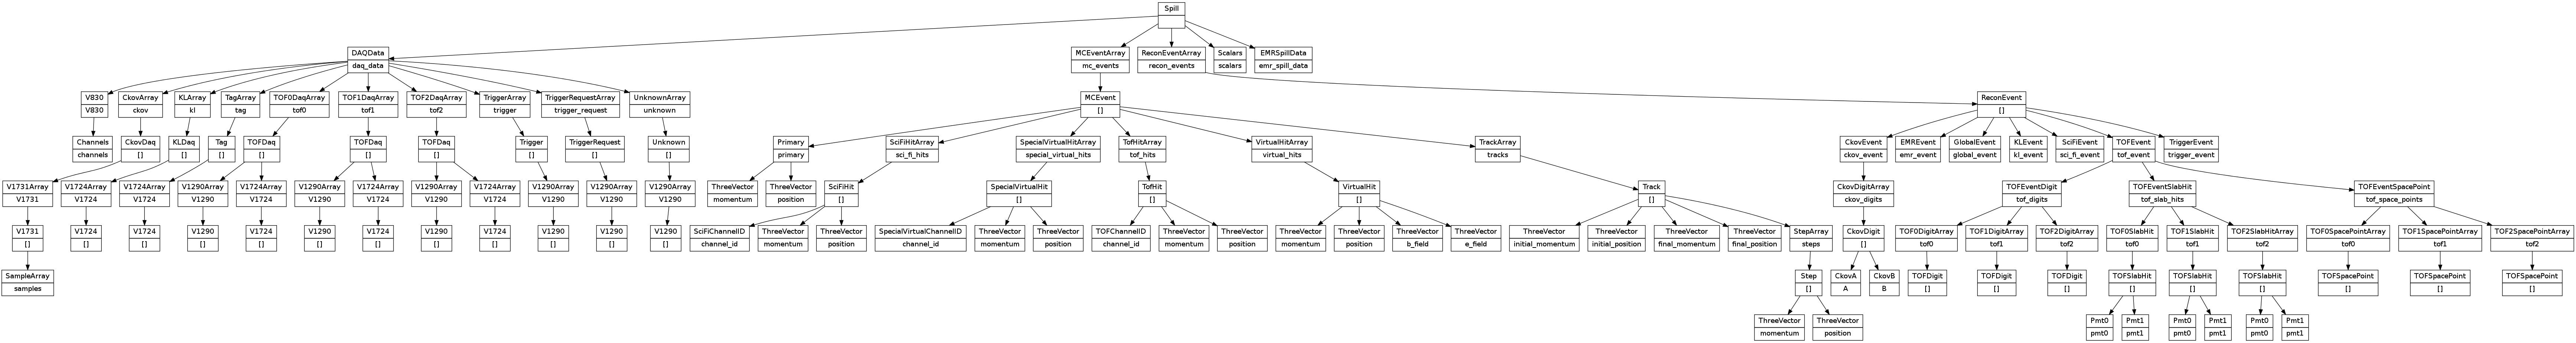
\includegraphics[width=0.9\textwidth]{data_structure.png}
\caption{The MAUS output data structure. The top label in each box is the name of the C++ class and the bottom label is the json branch name. If a [] is shown, this indicates that child objects are array items.}
\end{figure}

The MCEvent is subdivided into sensitive detector hits and some pure Monte Carlo outputs. The primary that led to data being created is held in the Primary branch. Here the random seed, primary position momentum and so forth is stored. Sensitive detector hits have Hit data (energy deposited, position, momentum, etc) and a detector specific ChannelId that represents the channel of the detector that was hit - e.g. for TOF this indexes the slab, plane and station. Virtual hits are also stored - these are not sensitive detector hits, rather output position, momenta etc of particles that cross a particular plane in space, time or proper time is recorded. Note virtual hits do not inherit from the Hit class and have a slightly different data structure.

The ReconEvent and DAQEvents are subdivided by detector. ReconEvents contain reconstructed particle data for each detector and the trigger. There is an additional branch that contains global reconstruction output, that is the track fitting between detectors.

The data can be written in two formats. The main data format is a ROOT binary format. This requires the ROOT package to read and write, which is a standard analysis/plotting package in High Energy Physics and is installed by the MAUS build script. The secondary data format is JSON. This is an ascii data-tree format that in principle can be read by any text editor. Specific JSON parsers are also available - for example, the python \emph{json} module is available and comes prepackaged with MAUS.

\section{Accessing ROOT files}
For details on how to access the ROOT files, please see the introduction section of this document.

\section{Conversion to, and Working With, JSON}
MAUS also provides output in the JSON data format. This is an ascii format with IO libraries available for C++, Python and other languages. Two utilities are provided to perform conversions, \verb|bin/utilities/json_to_root.py| and \verb|bin/utilities/root_to_json.py| for conversion from and to JSON format respectively. JSON Input and Output modules are provided, \verb|InputPyJson| and \verb|OutputPyJson|.

An example json analysis is available in \verb|bin/examples/load_json_file.py|/

\section{Extending the Data Structure}
The data structure can be extended in MAUS by adding extra classes to the existing data structure. The data classes are in \verb|src/common_cpp/DataStructure|. In order to make these classes accessible to ROOT, the following steps must be taken:
\begin{itemize}
\item Add a new class in \verb|src/common_cpp/DataStructure|.
\item Ensure that default constructor, copy constructor, equality operator and destructor is present. The destructor must be virtual.
\item Make a typedef for each type of STL object you wish to use. ROOT does not handle STL objects terribly well otherwise. Even then there are limitations, for example accessing STL vector objects can cause a segmentation fault in PyROOT. Specific accessors are required to access data from STL objects for PyROOT interface.
\item Add a call to the ClassDef() macro at the end of the class definition before the closing braces. The ClassDef() macro is defined by the ROOT \verb|Rtypes.h| header file, and generates metaclasses based on information in the class which is put into the (dynamically generated) \verb|MausDataStructure.h| class.
\item Add the class to the list of classes in \verb|src/common_cpp/DataStructure/LinkDef.hh|. This is required for the class to be linked properly to the main library, and a linker error will result if this step is not taken.
\end{itemize}
In order to make these classes accessible to JSON, it is necessary to add a new processor in \verb|src/common_cpp/JsonCppProcessors|. There are a few default processors available.
\begin{itemize}
\item \verb|src/common_cpp/JsonCppProcessors/ProcessorBase.hh| contains IProcessor pure interface class for all processors and ProcessorBase base class (which may contain some implementation)
\item \verb|src/common_cpp/JsonCppProcessors/PrimitivesProcessors.hh| contains processors for primitive types; BoolProcessor, IntProcessor, UIntProcessor, StringProcessor, DoubleProcessor
\item \verb|src/common_cpp/JsonCppProcessors/ArrayProcessors.hh| contains processors for array types. Two processors are available: PointerArrayProcessor which converts an STL vector of pointers to data; and ValueArrayProcessor which converts an STL vector of values to data.
\item \verb|src/common_cpp/JsonCppProcessors/ObjectProcessor.hh| contains a processor for object types. Most of the classes in the MAUS data structure are represented in JSON as objects (string value pairs) where each string names a branch and each value contains data, which may be another class.
\item \verb|src/common_cpp/JsonCppProcessors/ObjectMapProcessors.hh| contains a processor for converting from JSON objects to STL maps. This is useful for JSON objects that contain lots of branches all of the same type.
\end{itemize}

A script, \verb|bin/user/json_branch_to_data_structure_and_cpp_processor.py| is available that analyses a JSON object or JSON tree of nested objects and converts to C++ classes. The script is provided "as-is" and it is expected that developers will check the output, adding comments and tests where appropriate.

